\chapter{Related Work}
\label{ch:related_work}
This chapter describes the current state of the stepper motor controllers in the Robotics \& \acs{ai} group and the efforts to improve it.
Ongoing efforts to develop embedded systems in the Rust programming language are also described, both in the context of our research group and also in general.
Finally, similar projects - either software or hardware-wise are reported.

\section{KM2}
\label{sec:km2}
Nowadays, a second generation of the KM2 stepper motor controller is widely in use in the Robotics and \acs{ai} research group.
It is used primarily by the students of the BPC-PRP course for driving a simple differentially driven robot.
A render of the KM2 controller can be seen in the Figure~\ref{fig:km2render}.
The controller utilizes an ATMega8 paired with two stepper motor controllers DRV8825, that are utilized in the form of breakout boards generally used in the now obsolete 3D printer controlling RAMPS boards.
The motor controller is controlled using the I\textsuperscript{2}C bus.
There are two major shortcomings of the driver - the used \acs{mcu}'s I\textsuperscript{2}C peripheral's clock-stretching is not compatible with Raspberry Pi's, causing problems on clock speeds higher than 30 kHz.
The second shortcoming are the used driver chips which are quite loud and do not support contemporary advanced features.
Overheating is also common with them.

\begin{figure}[H]
    \centering
    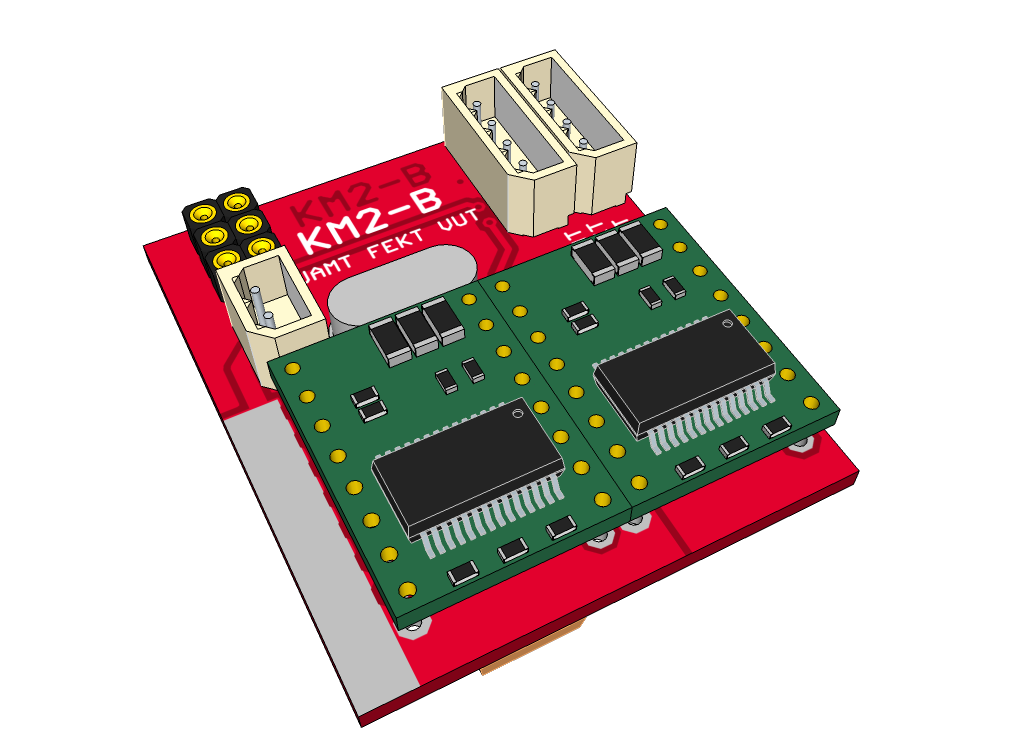
\includegraphics[width=0.5\textwidth]{obrazky/km2render}
    \caption{KM2 motor controller render~\cite{burian_km2renderpng_nodate}.}
    \label{fig:km2render}
\end{figure}

\newpage
\section{KM3}
\label{sec:km3}
The KM3 (or KM2-C) was supposed to be a successor to the previously described KM2 controller, and its main goal was to solve the clock stretching problem by utilizing an STM32F031 \acs{mcu}.
Another advantage of this revision was that the breakout boards for motor driver chips were replaced with driver chips soldered directly on the driver \acs{pcb}.
The controller can be seen in the Figure~\ref{fig:km3}.
Even though the new STM32F031 \acs{mcu} was an improvement over the ATMega8, it proved to be the bottleneck for implementing new functionality for the motor controller as the \acs{mcu} has very limited memory, both FLASH and \acs{ram} and also limited peripherals.
An example of these limitations being that the lack of pins made it impossible to directly generate pulses to control the STEP/DIR interface of the motor driver \acs{ic}; therefore the control had to be done manually in the software.
Another problem with this design is that the MCU utilizes a Cortex-M0 core, which means that the support for atomic instructions is missing, making it hard to work with guarantees about memory safety in cases of interrupt routine being called during memory manipulation.

We developed the Rust firmware~\cite{hybl_robotics-butkm3-rs_2020} for this board and concluded that the board and its design might be suitable for the students' robot projects, but it is way too limited to be used in more serious and complex projects.
We also concluded that the hardware and the technology it has been designed upon, as well as its goals, are obsolete, and that we should not pursue the development of this board further.

\begin{figure}[H]
    \centering
    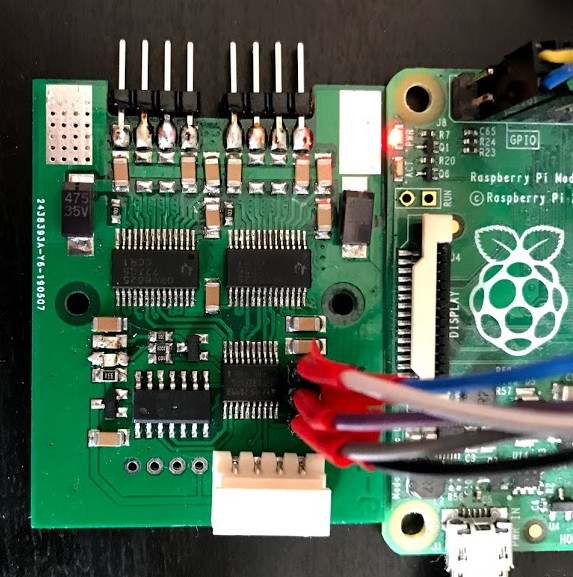
\includegraphics[width=0.5\textwidth]{obrazky/km3}
    \caption{The KM3 motor controller connected to a Raspberry Pi.}
    \label{fig:km3}
\end{figure}

\section{DCMotor}
\label{sec:dcmotor}
The DCMotor is a \acs{dc} (\acl{dc}) motor controller, developed in the Robotics \& \acs{ai} research group.
It was designed for feedback control of \acs{dc} motors, primarily \acs{dc} motors manufactured by Maxon.
The main design goal was to provide a cheaper alternative to the Maxon EPOS motor controllers.
The driver alongside a connected Maxon DC motor can be seen in the Figure~\ref{fig:dcmotor}.
Originally, the firmware for the motors, developed by Ing. František Burian, Ph.D., implemented current control and velocity control.
However, the firmware exhibited unwanted behavior, such as high motor temperature rises and unwanted high-pitch noise.
After consulting the problem with Ing. Lukáš Kopečný Ph.D., we decided to rewrite the firmware in Rust and remove the current controller, with the reasoning that current control of such low inductance motor makes not much sense, and instead, we replaced it with current limiting and failsafe overcurrent motor disabling.
The new firmware, and some hardware modifications were successfully deployed to seven DCMotor drivers as part of the exhibition robots for the Technical Museum in Brno, where they worked better than with the original firmware.

This driver was the first embedded project that used the Rust programming language to develop the firmware.
We believe that using the language was the right choice and made the firmware simpler to use and made it possible to develop it in such short time.
It can be said, that the work on the firmware for this board laid the foundation for the work on this thesis.

\begin{figure}[H]
    \centering
    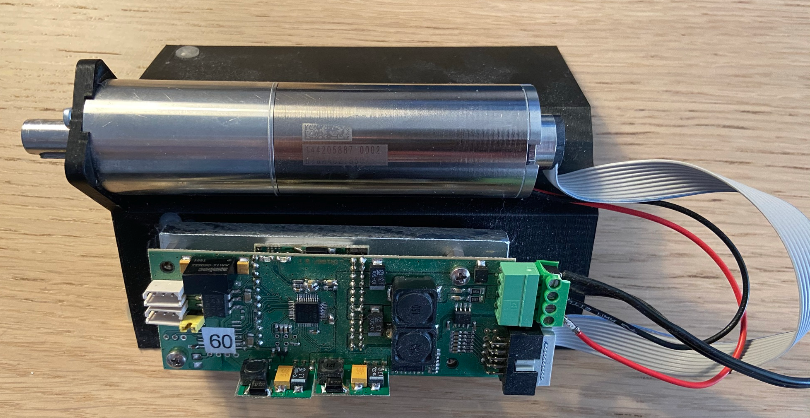
\includegraphics[width=0.7\textwidth]{obrazky/dcmotor}
    \caption{The DC Motor driver with a connected Maxon DC motor.}
    \label{fig:dcmotor}
\end{figure}

\newpage
\section{Mechaduino}
\label{sec:mechaduino}
Mechaduino is a project that aims to create a feedback-controlled servo motor out of a stepper motor.
The creators achieve that by mounting a PCB on the back of the motor that contains the power stage, a \acs{mcu}, and a 14-bit magnetic encoder~\cite{tropical_labs_mechaduino_2021}.
The mounting on the back of the stepper motor can be seen in the figure~\ref{fig:mechaduino}.
The big advantage that this project brings is the integration of the whole system de-facto into the motor, removing any need for a separate controller board.
On the other hand, the controller doesn't leverage any existing stepper motor controller solution and instead implements the winding control manually.
When compared to our proposed solution, the Mechaduino has many advantages even though it is only capable of controlling only one motor, it contains an encoder for feedback control and implements servo control algorithms out of the box.
On the other hand, our proposed solution leverages a state-of-the-art stepper motor controller \acs{ic}s (\acl{ic}), making it potentially less error-prone and better for future use and development.
If a semestral thesis and preliminary market research was preceding this project, the Mechaduino would provide valuable information to improve the design of our project.

\begin{figure}[H]
    \centering
    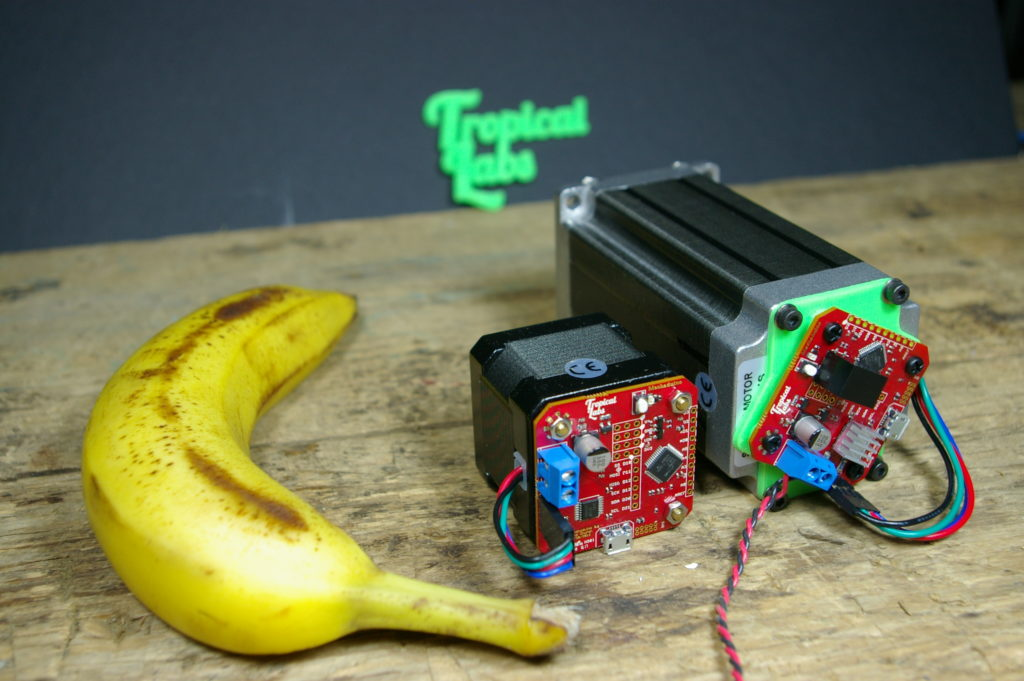
\includegraphics[width=0.7\textwidth]{obrazky/mechaduino}
    \caption{The Mechaduino controller boards mounted on the back of a stepper motors~\cite{tropical_labs_mechaduino_2021}.}
    \label{fig:mechaduino}
\end{figure}

\newpage
\section{Flott}
\label{sec:flott}
Flott is a set of libraries suitable for developing motion controllers programmed in the Rust programming language\cite{braun_flott_nodate}.
It is a relatively new project, and as of now, it contains an abstraction layer for stepper motors and acceleration ramp generators.
The project is taking a different approach to controlling the stepper motors we are.
It aims to utilize software pulse generation instead of timers and uses a variable step period in ramp generation.
Even though this is a good approach, we chose not to follow this model and instead implement this asynchronously using the \acs{mcu} peripherals.
On the other hand, the Flott project might be a great source of inspiration for future development, and maybe sometimes the SM4 motor controller might utilize it.

\section{Takeaways from Related Work}
\label{sec:related-work-takeaways}
The past stepper motor development efforts in the Robotics \& \acs{ai} research group showed the current solutions weak spots and advantages, which resulted in the following directions of the development of this project:
\begin{itemize}
    \item The project shall use a powerful, modern, and capable \acs{mcu} to fully support various features of the controller even in the future.
    \item The project shall use the state-of-art motor controller \acs{ic}s.
    \item The project shall use the Rust programming language for firmware and control software development.
\end{itemize}

The \acs{dc} Motor project showed us that writing a fully functional embedded firmware is possible and viable option.

The Mechaduino project serves as a great inspiration for what can be achieved in a servo motor based on a stepper motor.

Flott shows us that more people are trying to achieve building motion controllers in Rust and that we can get inspired from them and share knowledge with them.
We've been in contact with the Flott creator and consulted some ideas with them.
